%% my-first-homemade-linux-distro.tex
%% Copyright 2015 Gaël PORTAY <gael.portay@gmail.com>
%
% This work may be distributed and/or modified under the
% conditions of the LaTeX Project Public License, either version 1.3
% of this license or (at your option) any later version.
% The latest version of this license is in
%   http://www.latex-project.org/lppl.txt
% and version 1.3 or later is part of all distributions of LaTeX
% version 2005/12/01 or later.
%
% This work has the LPPL maintenance status `maintained'.
%
% The Current Maintainer of this work is Gaël PORTAY.
%
% This work consists of the file my-first-homemade-linux-distro.tex.

\documentclass[a4paper]{article}
\usepackage{caption}
\usepackage{graphicx}
\usepackage{hyperref}
\usepackage{listings}
\usepackage{subcaption}
\usepackage[T1]{fontenc}
\usepackage[utf8]{inputenc}
\usepackage[francais]{babel}

\lstloadlanguages{[ANSI]C,sh,make}

\title{Ma première distribution Linux faite maison}
\author{Gaël PORTAY}
\date{\today}

\begin{document}
%\sloppy
\maketitle

\begin{abstract}
\end{abstract}

\clearpage
\tableofcontents

\clearpage
\part{Le noyau}

\section{Première compilation}

%\begin{figure}
%\label{makefile_linux_download}
%\lstset{language=make,numbers=left,tabsize=2}
%\begin{lstlisting}
%kernel_download linux_download:
%	wget -qO- https://www.kernel.org/index.html\
%		| sed -n '/<td id="latest_link"/,/<\/td>/s,.*<a.*href="\(.*\)">\(.*\)</a>.*,wget -qO- \1\
%		| tar xvJ \&\& ln -sf linux-\2 linux,p'\$\
%		| sh
%\end{lstlisting}
%\caption{Makefile : règle toute faite pour télécharger et extraire la dernière version stable du noyau Linux.}
%\end{figure}

Entrons directement dans le vif du sujet et attaquons par la compilation du noyau !\\

\underline{Remarque} : je n'aborderai pas ici les concepts de la \textit{compilation croisée}. «~La compilation quoi ?!? croisée ?!?~». Bon, le plus simple c'est d'aller sur \href{https://fr.wikipedia.org/wiki/Compilateur#Compilation_crois.C3.A9e}{Wikipédia}. En gros, on compile quelque chose pour une architecture\footnote{Par architecture, comprenez processeur.}  cible autre que celle sur laquelle on est entrain de compiler. Vous y êtes toujours pas ?!? Plus simplement, on compile quelque chose sur notre PC \textit{Intel} (\textit{x86}) destiné à être utiliser sur notre \textit{Raspberry-PI} flambant neuf (\textit{ARM}). C'est bon vous y êtes ?!? Avec un exemple c'est toujours plus facile à comprendre...\\

Nous allons simplement compiler un noyau pour l'architecture (la machine) sur laquelle vous travaillez actuellement. Nous émulerons le noyau par la suite avec \textit{QEMU}.\\

Allons sur le site \href{http://www.kernel.org}{kernel.org} pout télécharger la dernière version stable du noyau\footnote{A l'heure où j'écris ces lignes, la dernière version stable du noyau est la version 4.3.}. La figure~\ref{makefile_linux_download} montre une règle \textit{Makefile} permettant d'automatiser le téléchargement et le désarchivage de la dernière version stable du noyau. Vous pouvez la réutiliser en faisant un copier/coller dans un fichier \textit{Makefile} et ensuite executer la commande suivante : \lstset{language=sh}\lstinline{make linux_download}.\\

\begin{verbatim}
kernel_download linux_download:
	wget -qO- https://www.kernel.org/index.html\
		| sed -n '/<td id="latest_link"/,/<\/td>/s,.*<a.*href="\(.*\)">\(.*\)</a>.*,wget -qO- \1 | tar xvJ \&\& ln -sf linux-\2 linux,p'\$\
		| sh
\end{verbatim}

%\begin{figure}
\label{make_linux_download}
\begin{verbatim}
$ make linux_download 
wget -qO- https://www.kernel.org/index.html | sed -n '/<td id="latest_link"/,/<\/td>/s,.*<a.*href="\(.*\)">\(.*\)</a>.*,wget -qO- \1 | tar xvJ \&\& ln -sf linux-\2 linux,p' | sh
linux-4.3/
linux-4.3/.get_maintainer.ignore
linux-4.3/.gitignore
linux-4.3/.mailmap
(...)
linux-4.3/virt/kvm/kvm_main.c
linux-4.3/virt/kvm/vfio.c
linux-4.3/virt/kvm/vfio.h
\end{verbatim}
%\caption{Makefile : une règle toute faite pour télécharger et extraire la dernière version stable du noyau Linux.}
%\end{figure}

Pour le reste de ce tutoriel, nous supposons que les fichiers sources sont dans le repertoire \textbf{./linux}.\\

Nous y voilà, nous somme fin prêt pour compiler notre premier noyau, exitez non ? Allez, on est parti. Ouvrez un terminal, si ce n'est pas déjà fait, et lancez la commande : \lstset{language=sh}\lstinline{cd linux && make}... et...

\begin{verbatim}
$ make
  HOSTCC  scripts/basic/fixdep
  HOSTCC  scripts/kconfig/conf.o
  SHIPPED scripts/kconfig/zconf.tab.c
  SHIPPED scripts/kconfig/zconf.lex.c
  SHIPPED scripts/kconfig/zconf.hash.c
  HOSTCC  scripts/kconfig/zconf.tab.o
  HOSTLD  scripts/kconfig/conf
scripts/kconfig/conf  --silentoldconfig Kconfig
***
*** Configuration file ".config" not found!
***
*** Please run some configurator (e.g. "make oldconfig" or
*** "make menuconfig" or "make xconfig").
***
scripts/kconfig/Makefile:37: recipe for target 'silentoldconfig' failed
make[2]: *** [silentoldconfig] Error 1
Makefile:531: recipe for target 'silentoldconfig' failed
make[1]: *** [silentoldconfig] Error 2
  SYSTBL  arch/x86/entry/syscalls/../../include/generated/asm/syscalls_32.h
  SYSHDR  arch/x86/entry/syscalls/../../include/generated/uapi/asm/unistd_32.h
  SYSHDR  arch/x86/entry/syscalls/../../include/generated/uapi/asm/unistd_64.h
  SYSHDR  arch/x86/entry/syscalls/../../include/generated/uapi/asm/unistd_x32.h
  HOSTCC  arch/x86/tools/relocs_32.o
  HOSTCC  arch/x86/tools/relocs_64.o
  HOSTCC  arch/x86/tools/relocs_common.o
  HOSTLD  arch/x86/tools/relocs
make: *** No rule to make target 'include/config/auto.conf', needed by 'include/config/kernel.release'.  Stop.
\end{verbatim}

C'était trop beau pour être vrai... compiler son noyau n'est pas aussi simple ! Linux est une noyau \textit{monolithyque} \textit{modulaire} qui supporte plusieurs \textit{plateformes} (promis, je ne voulais pas offenser). Comprenez simplement que le projet a besoin d'être configuré pour pouvoir être compilé avec un vulgaire \lstset{language=sh}\lstinline{make}.\\

\section{Configuration}

Linux utilise le language \textit{\href{https://www.kernel.org/doc/Documentation/kbuild/kconfig-language.txt}{Kconfig}} pour décrire les options de configurations : ce sont les fichiers \textbf{Kconfig} présent un peu partout dans les sources.\\

Il existe plusieurs \textit{front-ends} (ou interfaces) pour afficher le menu de configuration du noyau. Généralement, les développeurs utilisent la vielle interface en \textit{ncurses} que l'on appel via \lstset{language=sh}\lstinline{make menuconfig}. Il existe également \textbf{config} (ligne de commande), \textbf{nconfig} (ncurses), \textbf{xconfig} (Qt) et \textbf{gconfig} (GTK+).\\

Vous avez surement remarqué le message suivant lorsque la première commande \lstset{language=sh}\lstinline{make} a échouée :
\begin{verbatim}
***
*** Configuration file ".config" not found!
***
*** Please run some configurator (e.g. "make oldconfig" or
*** "make menuconfig" or "make xconfig").
***
\end{verbatim}

Le fichier \textbf{.config}, qui contient la configuration du noyau, est manquant ! Ce fichier est une simple définition des options qui seront compilés ou non, intégré à l'image du noyau ou disponible via une module. Bien entendu, les sources du noyau viennent sans aucune configuration. Il va donc falloir générer cette configuration.\\

\subsection{menuconfig}

\begin{figure}
\label{fig:make_menuconfig}
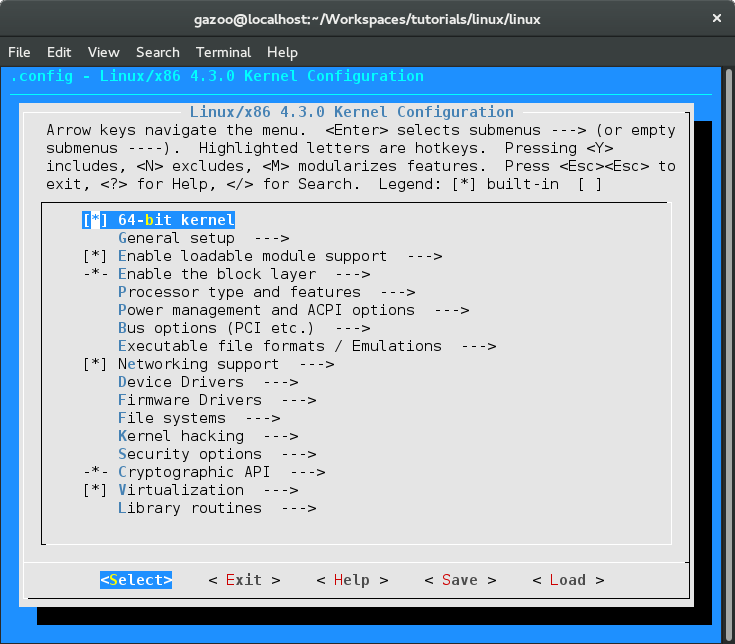
\includegraphics[scale=0.5]{make-menuconfig.png}
\caption{make - menuconfig}
\end{figure}

Allez, on se fait une petite frailleur ?!? Executez la commande \lstinline{make menuconfig}\footnote{Nous avons besoin du paquet de developpement de ncurses. Si vous n'y arrivez pas, passez simplement cette partie.}. La figure~\ref{fig:make_menuconfig} montre le menu principal de configuration du noyau. Vous pouvez vous ballader dans les sous menus avec les flèches haut et bas, entrez dans les sous menu avec la touche Entrée, revenir au menu précédent avec la touche Echap, cocher/décocher avec la touche Espace. Quittez sans sauvegarder \textit{Ctrl-C} et \textit{No}\footnote{Si vous avez malencontreusement sauvegarder, supprimez le fichier \textbf{.config} via \lstset{language=sh}\lstinline{rm .config}}.

\begin{verbatim}
$ make menuconfig
ou
$ make tinyconfig
\end{verbatim}

\section{tinyconfig}

Nous allons créer une configuration minimal. Pour cela, nous allons invoquer la regle tinyconfig.

\begin{verbatim}
$ make tinyconfig
scripts/kconfig/conf  --allnoconfig Kconfig
#
# configuration written to .config
#
Using .config as base
Merging ./kernel/configs/tiny.config
Value of CONFIG_CC_OPTIMIZE_FOR_SIZE is redefined by fragment ./kernel/configs/tiny.config:
Previous value: # CONFIG_CC_OPTIMIZE_FOR_SIZE is not set
New value: CONFIG_CC_OPTIMIZE_FOR_SIZE=y

Value of CONFIG_KERNEL_XZ is redefined by fragment ./kernel/configs/tiny.config:
Previous value: # CONFIG_KERNEL_XZ is not set
New value: CONFIG_KERNEL_XZ=y

Value of CONFIG_OPTIMIZE_INLINING is redefined by fragment ./kernel/configs/tiny.config:
Previous value: # CONFIG_OPTIMIZE_INLINING is not set
New value: CONFIG_OPTIMIZE_INLINING=y

Value of CONFIG_SLOB is redefined by fragment ./kernel/configs/tiny.config:
Previous value: # CONFIG_SLOB is not set
New value: CONFIG_SLOB=y

Merging ./arch/x86/configs/tiny.config
Value of CONFIG_NOHIGHMEM is redefined by fragment ./arch/x86/configs/tiny.config:
Previous value: # CONFIG_NOHIGHMEM is not set
New value: CONFIG_NOHIGHMEM=y

#
# merged configuration written to ./.config (needs make)
#
scripts/kconfig/conf  --oldconfig Kconfig
.config:900:warning: override: KERNEL_XZ changes choice state
.config:902:warning: override: SLOB changes choice state
.config:903:warning: override: NOHIGHMEM changes choice state
*
* Restart config...
*
*
* Processor type and features
*
DMA memory allocation support (ZONE_DMA) [N/y/?] n
Symmetric multi-processing support (SMP) [N/y/?] n
Processor feature human-readable names (X86_FEATURE_NAMES) [N/y/?] n
Support for extended (non-PC) x86 platforms (X86_EXTENDED_PLATFORM) [N/y/?] n
Eurobraille/Iris poweroff module (X86_32_IRIS) [N/y/?] n
Single-depth WCHAN output (SCHED_OMIT_FRAME_POINTER) [N/y/?] n
*
* Linux guest support
*
Linux guest support (HYPERVISOR_GUEST) [N/y/?] n
Processor family
  1. 486 (M486)
  2. 586/K5/5x86/6x86/6x86MX (M586)
  3. Pentium-Classic (M586TSC)
  4. Pentium-MMX (M586MMX)
> 5. Pentium-Pro (M686)
  6. Pentium-II/Celeron(pre-Coppermine) (MPENTIUMII)
  7. Pentium-III/Celeron(Coppermine)/Pentium-III Xeon (MPENTIUMIII)
  8. Pentium M (MPENTIUMM)
  9. Pentium-4/Celeron(P4-based)/Pentium-4 M/older Xeon (MPENTIUM4)
  10. K6/K6-II/K6-III (MK6)
  11. Athlon/Duron/K7 (MK7)
  12. Opteron/Athlon64/Hammer/K8 (MK8)
  13. Crusoe (MCRUSOE)
  14. Efficeon (MEFFICEON)
  15. Winchip-C6 (MWINCHIPC6)
  16. Winchip-2/Winchip-2A/Winchip-3 (MWINCHIP3D)
  17. AMD Elan (MELAN)
  18. GeodeGX1 (MGEODEGX1)
  19. Geode GX/LX (MGEODE_LX)
  20. CyrixIII/VIA-C3 (MCYRIXIII)
  21. VIA C3-2 (Nehemiah) (MVIAC3_2)
  22. VIA C7 (MVIAC7)
  23. Core 2/newer Xeon (MCORE2)
  24. Intel Atom (MATOM)
choice[1-24]: 5
Generic x86 support (X86_GENERIC) [N/y/?] n
PentiumPro memory ordering errata workaround (X86_PPRO_FENCE) [N/y/?] n
*
* Supported processor vendors
*
Supported processor vendors (PROCESSOR_SELECT) [N/y/?] n
HPET Timer Support (HPET_TIMER) [N/y/?] n
Enable DMI scanning (DMI) [N/y/?] n
Preemption Model
> 1. No Forced Preemption (Server) (PREEMPT_NONE)
  2. Voluntary Kernel Preemption (Desktop) (PREEMPT_VOLUNTARY)
  3. Preemptible Kernel (Low-Latency Desktop) (PREEMPT)
choice[1-3]: 1
Local APIC support on uniprocessors (X86_UP_APIC) [N/y/?] n
Machine Check / overheating reporting (X86_MCE) [N/y/?] n
Legacy VM86 support (X86_LEGACY_VM86) [N/y/?] n
Toshiba Laptop support (TOSHIBA) [N/y/?] n
Dell i8k legacy laptop support (I8K) [N/y/?] n
Enable X86 board specific fixups for reboot (X86_REBOOTFIXUPS) [N/y/?] n
CPU microcode loading support (MICROCODE) [N/y/?] n
/dev/cpu/*/msr - Model-specific register support (X86_MSR) [N/y/?] n
/dev/cpu/*/cpuid - CPU information support (X86_CPUID) [N/y/?] n
High Memory Support
> 1. off (NOHIGHMEM)
  2. 4GB (HIGHMEM4G)
  3. 64GB (HIGHMEM64G)
choice[1-3]: 1
Memory split
> 1. 3G/1G user/kernel split (VMSPLIT_3G)
  2. 3G/1G user/kernel split (for full 1G low memory) (VMSPLIT_3G_OPT)
  3. 2G/2G user/kernel split (VMSPLIT_2G)
  4. 2G/2G user/kernel split (for full 2G low memory) (VMSPLIT_2G_OPT)
  5. 1G/3G user/kernel split (VMSPLIT_1G)
choice[1-5?]: 1
PAE (Physical Address Extension) Support (X86_PAE) [N/y/?] (NEW) 
Memory model
> 1. Flat Memory (FLATMEM_MANUAL)
  2. Sparse Memory (SPARSEMEM_MANUAL)
choice[1-2]: 1
Allow for memory compaction (COMPACTION) [N/y/?] n
Enable KSM for page merging (KSM) [N/y/?] n
Low address space to protect from user allocation (DEFAULT_MMAP_MIN_ADDR) [4096] 4096
Transparent Hugepage Support (TRANSPARENT_HUGEPAGE) [N/y/?] n
Enable cleancache driver to cache clean pages if tmem is present (CLEANCACHE) [N/y/?] n
Contiguous Memory Allocator (CMA) [N/y/?] n
Common API for compressed memory storage (ZPOOL) [N/y/?] n
Low density storage for compressed pages (ZBUD) [N/y/?] n
Memory allocator for compressed pages (ZSMALLOC) [N/y/?] n
Check for low memory corruption (X86_CHECK_BIOS_CORRUPTION) [N/y/?] n
Amount of low memory, in kilobytes, to reserve for the BIOS (X86_RESERVE_LOW) [64] 64
MTRR (Memory Type Range Register) support (MTRR) [N/y/?] n
x86 architectural random number generator (ARCH_RANDOM) [N/y/?] n
Supervisor Mode Access Prevention (X86_SMAP) [N/y/?] n
Intel MPX (Memory Protection Extensions) (X86_INTEL_MPX) [N/y/?] n
Enable seccomp to safely compute untrusted bytecode (SECCOMP) [N/y/?] n
Timer frequency
  1. 100 HZ (HZ_100)
> 2. 250 HZ (HZ_250)
  3. 300 HZ (HZ_300)
  4. 1000 HZ (HZ_1000)
choice[1-4?]: 2
kexec system call (KEXEC) [N/y/?] n
Physical address where the kernel is loaded (PHYSICAL_START) [0x1000000] 0x1000000
Build a relocatable kernel (RELOCATABLE) [N/y/?] n
Alignment value to which kernel should be aligned (PHYSICAL_ALIGN) [0x200000] 0x200000
Disable the 32-bit vDSO (needed for glibc 2.3.3) (COMPAT_VDSO) [N/y/?] n
Built-in kernel command line (CMDLINE_BOOL) [N/y/?] n
Enable the LDT (local descriptor table) (MODIFY_LDT_SYSCALL) [N/y/?] n
#
# configuration written to .config
#
\end{verbatim}

Le noyau est maintenant configuré. Un fichier \textbf{.config} est créé à la racine du projet. Ce fichier contient une configuration strictement minimale, et nous allons pouvoir le compiler avec \lstset{language=sh}\lstinline{make}.\\

\begin{verbatim}
$ make
  GEN     ./Makefile
scripts/kconfig/conf  --silentoldconfig Kconfig
  SYSTBL  arch/x86/entry/syscalls/../../include/generated/asm/syscalls_32.h
  SYSHDR  arch/x86/entry/syscalls/../../include/generated/uapi/asm/unistd_32.h
  SYSHDR  arch/x86/entry/syscalls/../../include/generated/uapi/asm/unistd_64.h
  SYSHDR  arch/x86/entry/syscalls/../../include/generated/uapi/asm/unistd_x32.h
  HOSTCC  arch/x86/tools/relocs_32.o
  HOSTCC  arch/x86/tools/relocs_64.o
  HOSTCC  arch/x86/tools/relocs_common.o
  HOSTLD  arch/x86/tools/relocs
  CHK     include/config/kernel.release
  UPD     include/config/kernel.release
(...)
  LD      arch/x86/boot/setup.elf
  OBJCOPY arch/x86/boot/setup.bin
  OBJCOPY arch/x86/boot/vmlinux.bin
  HOSTCC  arch/x86/boot/tools/build
  BUILD   arch/x86/boot/bzImage
Setup is 15452 bytes (padded to 15872 bytes).
System is 342 kB
CRC 61bf4503
Kernel: arch/x86/boot/bzImage is ready  (#1)
\end{verbatim}

Notre noyau flambant neuf est disponible dans \textbf{linux/arch/x86/boot/vmlinuz.bin}.

\section{Emulation}

\begin{figure}
\label{qemu_first_run}
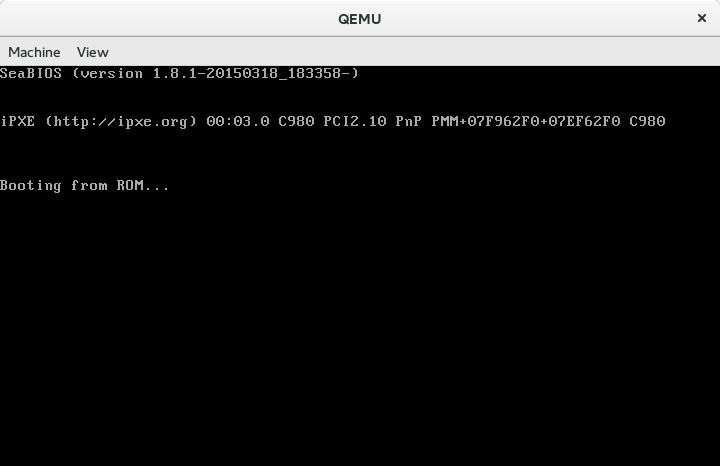
\includegraphics[scale=0.5]{qemu-first-run.png}
\caption{qemu-system-i386 - Console QEMU}
\end{figure}

Nous allons maintenant émuler notre noyau fraichement compilé avec \textit{QEMU} via la commande \lstset{language=sh}\lstinline{qemu-system-i386 -kernel arch/x86/boot/bzImage}. La figure~\ref{qemu_first_run} montre la console ouverte par \textit{QEMU}.\\

Vous l'aurez remarqué, il ne se passe rien. En effet, nous allons rendre le noyau verbeux et afficher les traces sur la console de \textit{QEMU}.

\subsection{Noyau verbeux}

\begin{figure}
\label{menuconfig_enable_printk}
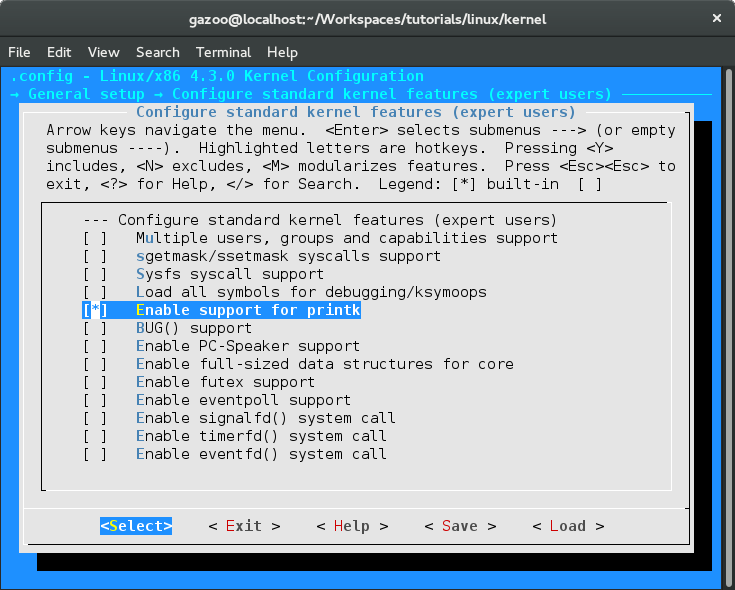
\includegraphics[scale=0.5]{menuconfig-enable-printk.png}
\caption{menuconfig - Support de printk}
\end{figure}

Pour rendre le noyau plus verbeux, nous allons activer les traces \textit{printk}. Sous le menu \textbf{General Setup}, puis \textbf{Configure standard kernel features (expert users)}, cochons la case \textbf{Enable support for printk} comme illustré par la figure~\ref{menuconfig_enable_printk}.\\

\begin{figure}
\label{menuconfig_enable_tty}
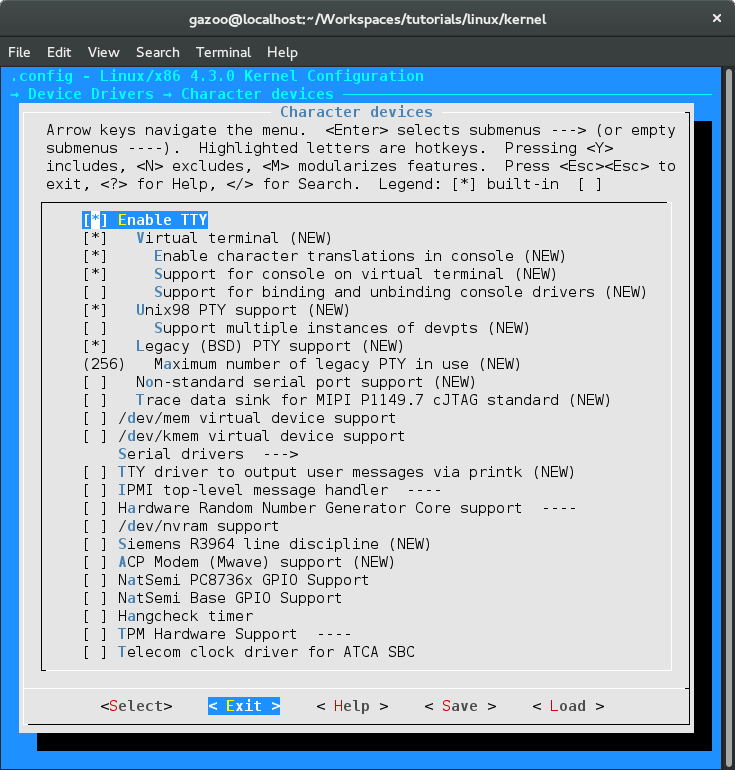
\includegraphics[scale=0.5]{menuconfig-enable-tty.png}
\caption{menuconfig - Support de TTY}
\end{figure}

\begin{figure}
\label{menuconfig_enable_console}
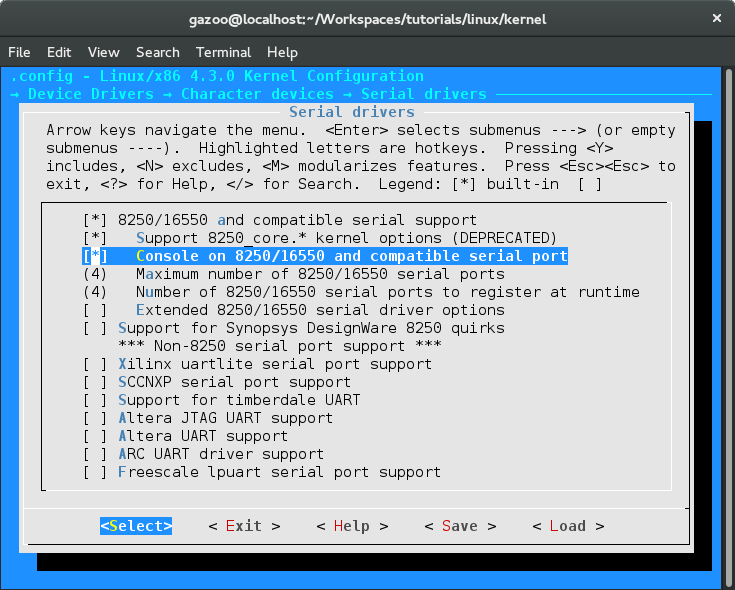
\includegraphics[scale=0.5]{menuconfig-enable-console-on-8250-16550-serial-port.png}
\caption{menuconfig - Support de la console sur les ports séries 8250/16550 (ou compatible)}
\end{figure}

Ensuite, nous allons configurer le projet pour compiler les pilotes utilisés par la console de \textit{QEMU}. Sous le menu \textbf{Device Drivers} puis \textbf{Character devices  --->}, cochons la case \textbf{Enable TTY}. Et, sous le nouveau sous-menu \textbf{Serial drivers  --->} cochons également la case \textbf{8250/16550 and compatible serial support} puis \textbf{Console on 8250/16550 and compatible serial port}. Referez vous aux figures~\ref{menuconfig_enable_console} et \ref{menuconfig_enable_tty}.\\

Deux nouveaux périphériques sont utilisables par le noyau :
\begin{itemize}
\item \textbf{console} et
\item \textbf{ttySx} ou \textit{x} représente un entier définissant le numéro du port série.
\end{itemize}

\subsection{QEMU}

Sur la ligne de commande de QEMU, nous devons spécifier deux nouveaux paramètres :
\begin{itemize}
\item le premier pour émuler un port série (\textit{char-device}) et
\item le second pour surcharger la ligne de commande du noyau afin de spécifier le port série émulé comme étant la console du noyau.
\end{itemize}

\subsubsection{Emulation d'un port série}

L'émulation du port série se traduit par une série de deux paramètres :
\begin{itemize}
\item la création du périphérique de type isa-serial : \lstset{language=sh}\lstinline{-device isa-serial,chardev=tty}
\item l'association \lstset{language=sh}\lstinline{-chardev stdio,id=tty}
\end{itemize}

\subsubsection{Surcharge de la ligne de commande du noyau}

Nous allons surcharger la ligne de commande du noyau en ajoutant une console via le paramètre \href{https://www.kernel.org/doc/Documentation/serial-console.txt}{\textbf{console=device,options}}.

\lstset{language=sh}\lstinline{-append console=ttyS0}

Et voilà !

\begin{verbatim}
$ qemu-system-i386 -kernel output/linux-x86/arch/x86/boot/bzImage -append "console=ttyS0" -serial stdio
Linux version 4.3.0 (gazoo@localhost.localdomain) (gcc version 5.1.1 20150618 (Red Hat 5.1.1-4) (GCC) ) #4 Mon Dec 7 17:18:49 CET 2015
x86/fpu: Legacy x87 FPU detected.
x86/fpu: Using 'lazy' FPU context switches.
e820: BIOS-provided physical RAM map:
BIOS-e820: [mem 0x0000000000000000-0x000000000009fbff] usable
BIOS-e820: [mem 0x000000000009fc00-0x000000000009ffff] reserved
BIOS-e820: [mem 0x00000000000f0000-0x00000000000fffff] reserved
BIOS-e820: [mem 0x0000000000100000-0x0000000007fdffff] usable
BIOS-e820: [mem 0x0000000007fe0000-0x0000000007ffffff] reserved
BIOS-e820: [mem 0x00000000fffc0000-0x00000000ffffffff] reserved
Notice: NX (Execute Disable) protection missing in CPU!
e820: last_pfn = 0x7fe0 max_arch_pfn = 0x100000
init_memory_mapping: [mem 0x00000000-0x000fffff]
init_memory_mapping: [mem 0x07800000-0x07bfffff]
init_memory_mapping: [mem 0x00100000-0x077fffff]
init_memory_mapping: [mem 0x07c00000-0x07fdffff]
127MB LOWMEM available.
  mapped low ram: 0 - 07fe0000
  low ram: 0 - 07fe0000
Zone ranges:
  Normal   [mem 0x0000000000001000-0x0000000007fdffff]
Movable zone start for each node
Early memory node ranges
  node   0: [mem 0x0000000000001000-0x000000000009efff]
  node   0: [mem 0x0000000000100000-0x0000000007fdffff]
Initmem setup node 0 [mem 0x0000000000001000-0x0000000007fdffff]
e820: [mem 0x08000000-0xfffbffff] available for PCI devices
clocksource: refined-jiffies: mask: 0xffffffff max_cycles: 0xffffffff, max_idle_ns: 7645519600211568 ns
Built 1 zonelists in Zone order, mobility grouping on.  Total pages: 32382
Kernel command line: console=ttyS0
PID hash table entries: 512 (order: -1, 2048 bytes)
Dentry cache hash table entries: 16384 (order: 4, 65536 bytes)
Inode-cache hash table entries: 8192 (order: 3, 32768 bytes)
Initializing CPU#0
Memory: 128016K/130552K available (730K kernel code, 96K rwdata, 112K rodata, 108K init, 196K bss, 2536K reserved, 0K cma-reserved)
virtual kernel memory layout:
    fixmap  : 0xfffe5000 - 0xfffff000   ( 104 kB)
    vmalloc : 0xc87e0000 - 0xfffe3000   ( 888 MB)
    lowmem  : 0xc0000000 - 0xc7fe0000   ( 127 MB)
      .init : 0xc10ee000 - 0xc1109000   ( 108 kB)
      .data : 0xc10b6cc9 - 0xc10ec0c0   ( 212 kB)
      .text : 0xc1000000 - 0xc10b6cc9   ( 731 kB)
Checking if this processor honours the WP bit even in supervisor mode...Ok.
NR_IRQS:16 nr_irqs:16 16
Console: colour VGA+ 80x25
console [ttyS0] enabled
tsc: Unable to calibrate against PIT
tsc: No reference (HPET/PMTIMER) available
tsc: Marking TSC unstable due to could not calculate TSC khz
Calibrating delay loop... 306.94 BogoMIPS (lpj=613888)
pid_max: default: 4096 minimum: 301
Mount-cache hash table entries: 1024 (order: 0, 4096 bytes)
Mountpoint-cache hash table entries: 1024 (order: 0, 4096 bytes)
Last level iTLB entries: 4KB 0, 2MB 0, 4MB 0
Last level dTLB entries: 4KB 0, 2MB 0, 4MB 0, 1GB 0
CPU: Intel QEMU Virtual CPU version 2.3.1 (family: 0x6, model: 0x6, stepping: 0x3)
Performance Events: Broken PMU hardware detected, using software events only.
Failed to access perfctr msr (MSR c2 is 0)
clocksource: jiffies: mask: 0xffffffff max_cycles: 0xffffffff, max_idle_ns: 7645041785100000 ns
clocksource: pit: mask: 0xffffffff max_cycles: 0xffffffff, max_idle_ns: 1601818034827 ns
clocksource: Switched to clocksource pit
platform rtc_cmos: registered platform RTC device (no PNP device found)
Serial: 8250/16550 driver, 4 ports, IRQ sharing disabled
serial8250: ttyS0 at I/O 0x3f8 (irq = 4, base_baud = 115200) is a 16550A
serio: i8042 KBD port at 0x60,0x64 irq 1
serio: i8042 AUX port at 0x60,0x64 irq 12
mousedev: PS/2 mouse device common for all mice
input: AT Translated Set 2 keyboard as /devices/platform/i8042/serio0/input/input0
input: ImExPS/2 Generic Explorer Mouse as /devices/platform/i8042/serio1/input/input3
Freeing unused kernel memory: 108K (c10ee000 - c1109000)
Kernel panic - not syncing: No working init found.  Try passing init= option to kernel. See Linux Documentation/init.txt for guidance.
Kernel Offset: disabled
---[ end Kernel panic - not syncing: No working init found.  Try passing init= option to kernel. See Linux Documentation/init.txt for guidance.
\end{verbatim}

Un noyau, c'est bien, mais ne consitue en rien un système complet : il manque la partie applicative user-space.

\url{http://nairobi-embedded.org/qemu_serial_terminal_redirection.html}

\part{User-space}

\clearpage
\appendix

\section{Kconfig}

\begin{verbatim}
# Un commentaire commence par un '#' (cette ligne est donc un commentaire).
#
# Une option est prefixée par 'CONFIG_'.
# Une option est typée et peut prendre les types suivants :
#  - bool
#  - integer
#  - string
#  - tristate

# type bool :
#  - y pour yes
#  - # CONFIG_xxx is not set : pour no
CONFIG_xxx = y
# CONFIG_xxx is not set

# type string :
CONFIG_xxx = "une chaine de caractères"

# Le type integer peut prendre une valeur entière,
# aussi bien sous forme décimale
CONFIG_xxx = 123
# qu'hexadécimale
CONFIG_xxx = 0xff

# type tristate : est utilisé pour les modules.
# Il peut prendre les 3 valeurs ci-dessous:
#  - y pour yes : compilé et intégré dans le noyau
#  - m pour module : compilé et peut être chargé (ou déchargé)
#                    via insmod/modprobe (ou rmmod)
#  - # CONFIG_xxx is not set : non compilé
CONFIG_xxx=y
CONFIG_xxx=m
# CONFIG_xxx is not set
\end{verbatim}

\clearpage
\listoffigures

\clearpage
\listoftables

\end{document}
